% !TeX root = ../main.tex

\section{Prozessablauf im Detail}

\begin{frame}{Prozessablauf im Detail}
    \begin{figure}
        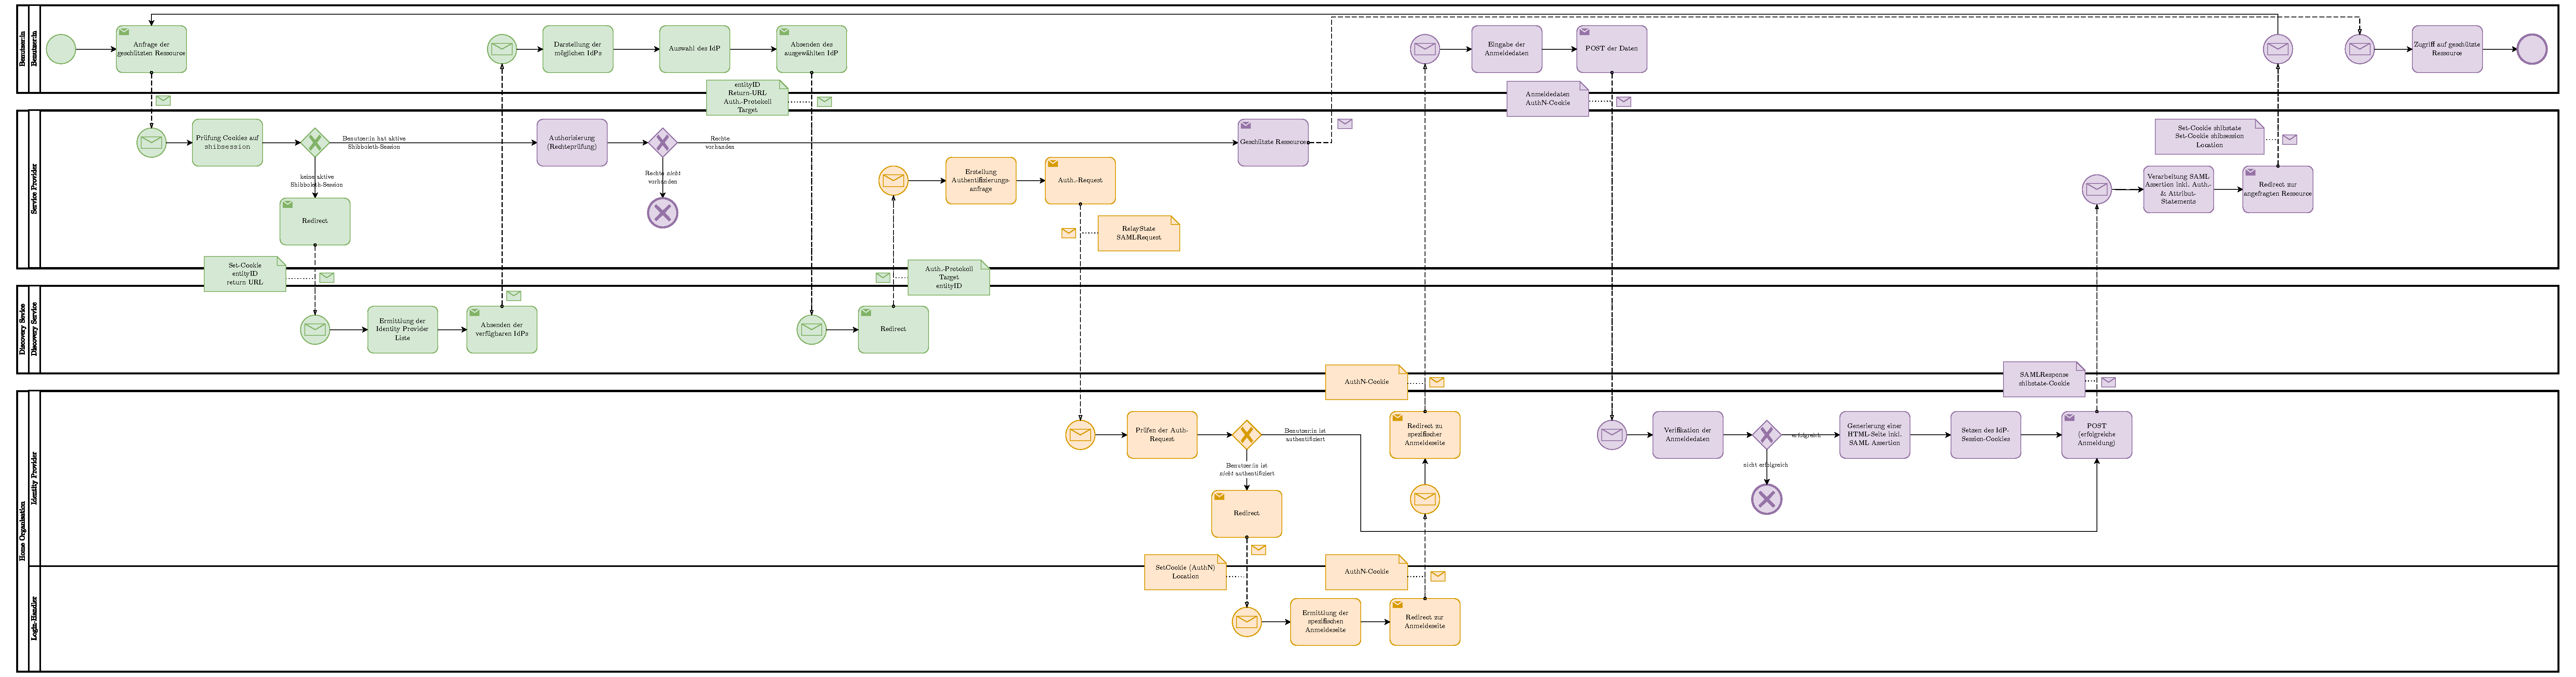
\includegraphics[width=\textwidth]{../assets/bis_bpmn.drawio.pdf}
        \caption{BPMN-Diagramm zum Login-Prozess mit Shibboleth~\cite[vgl.][]{switchExpertDemoSWITCHaai2024a}}
    \end{figure}        
\end{frame}


\begin{frame}{Phase 1: Erster Zugriff}
    \only<beamer>{
        \framezoom<1><2>[border](1.1cm,0.6cm)(5.15cm,3cm)
        \framezoom<1><3>[border](1.1cm,2.7cm)(5.15cm,3cm)
        \framezoom<1><4>[border](1.2cm,3.7cm)(5.15cm,3cm)

        \framezoom<1><5>[border](4.2cm,0.5cm)(5.15cm,3cm)
        \framezoom<1><6>[border](5.3cm,3.8cm)(5.15cm,3cm)
        \framezoom<1><7>[border](5.3cm,3.0cm)(5.15cm,3cm)
    }

    \begin{figure}
        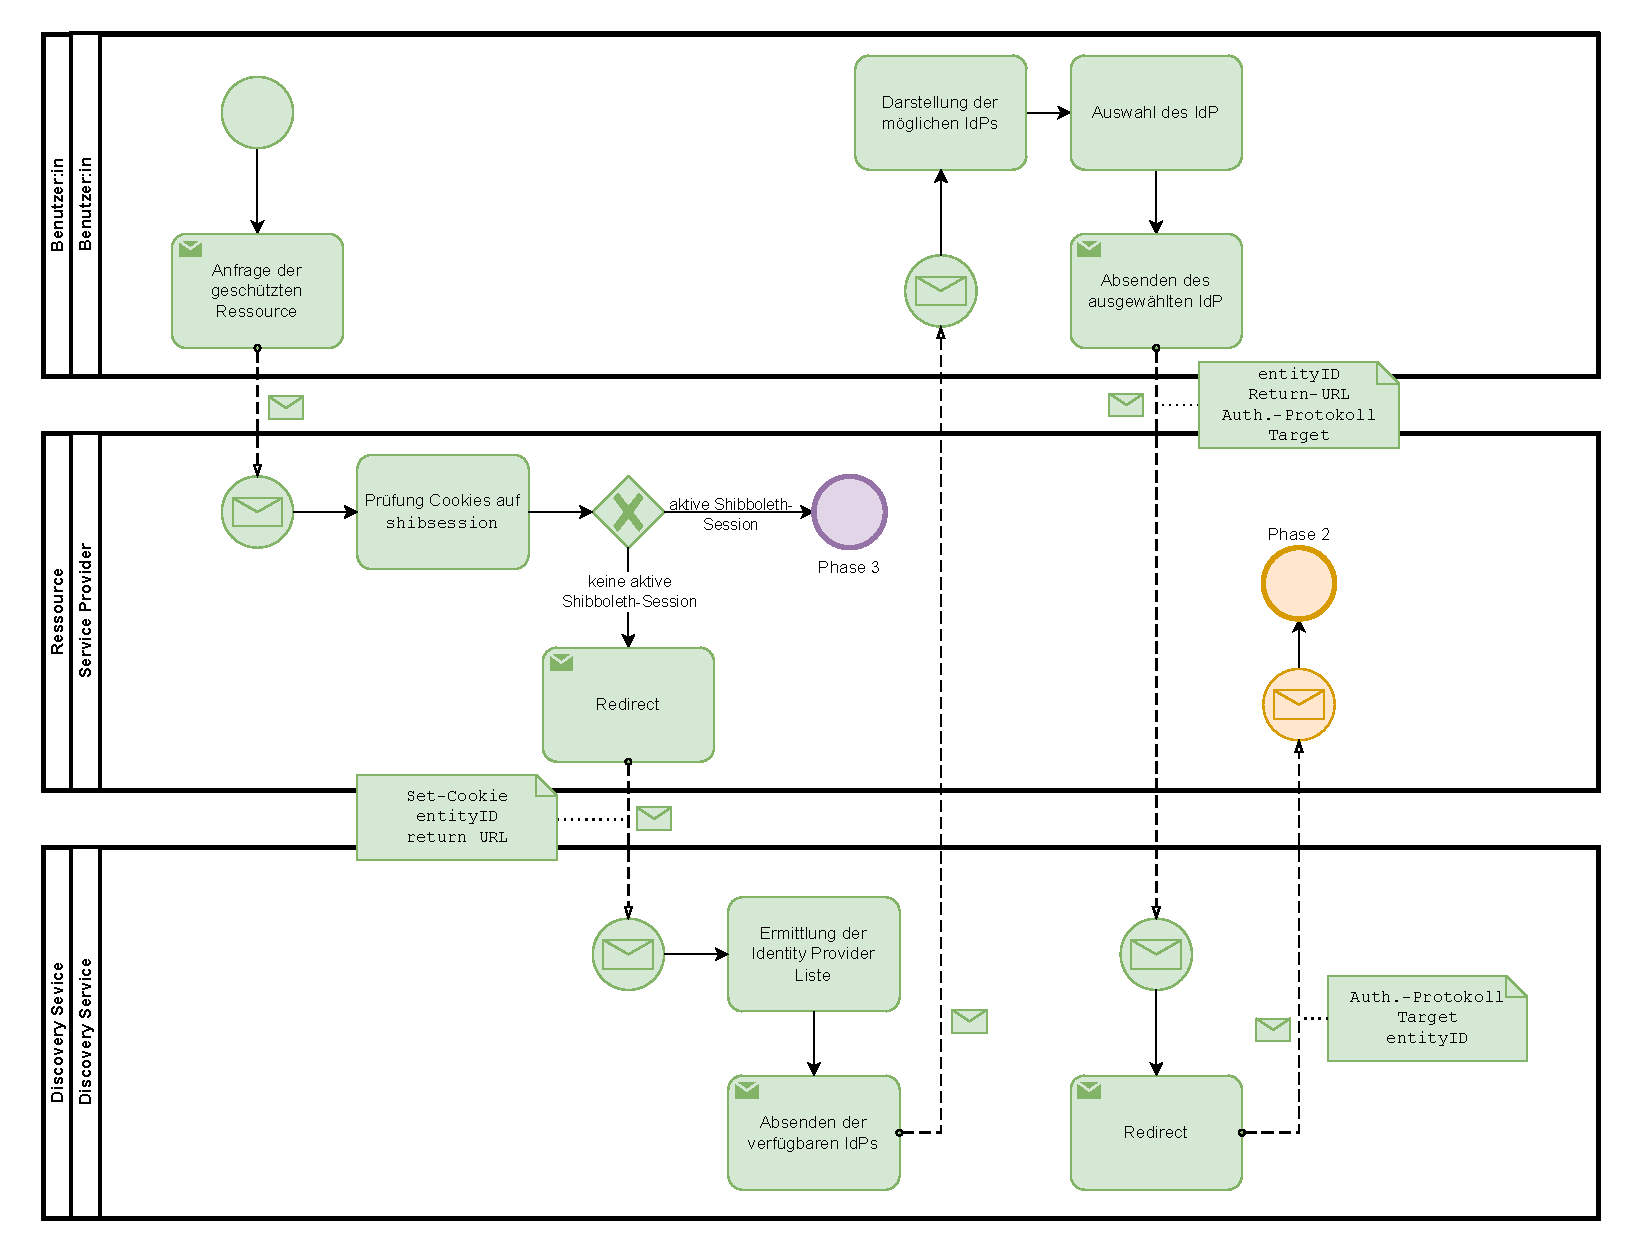
\includegraphics[height=0.7\paperheight]{../assets/bis_bpmn_phase_1.drawio.pdf}
        \caption{Phase 1 im Shibboleth-Prozess~\cite[vgl.][]{switchExpertDemoSWITCHaai2024a}}
    \end{figure}
\end{frame}


\begin{frame}{Phase 2: Session-Initialisierung \& Authentifizierungsanfrage}
    \only<beamer>{
        \framezoom<1><2>[border](1.3cm,1.2cm)(4.2cm,3cm)
        \framezoom<1><3>[border](3.8cm,3.8cm)(4.8cm,3cm)
        \framezoom<1><4>[border](4cm,0.2cm)(5.3cm,4.7cm)
    }

    \begin{figure}
        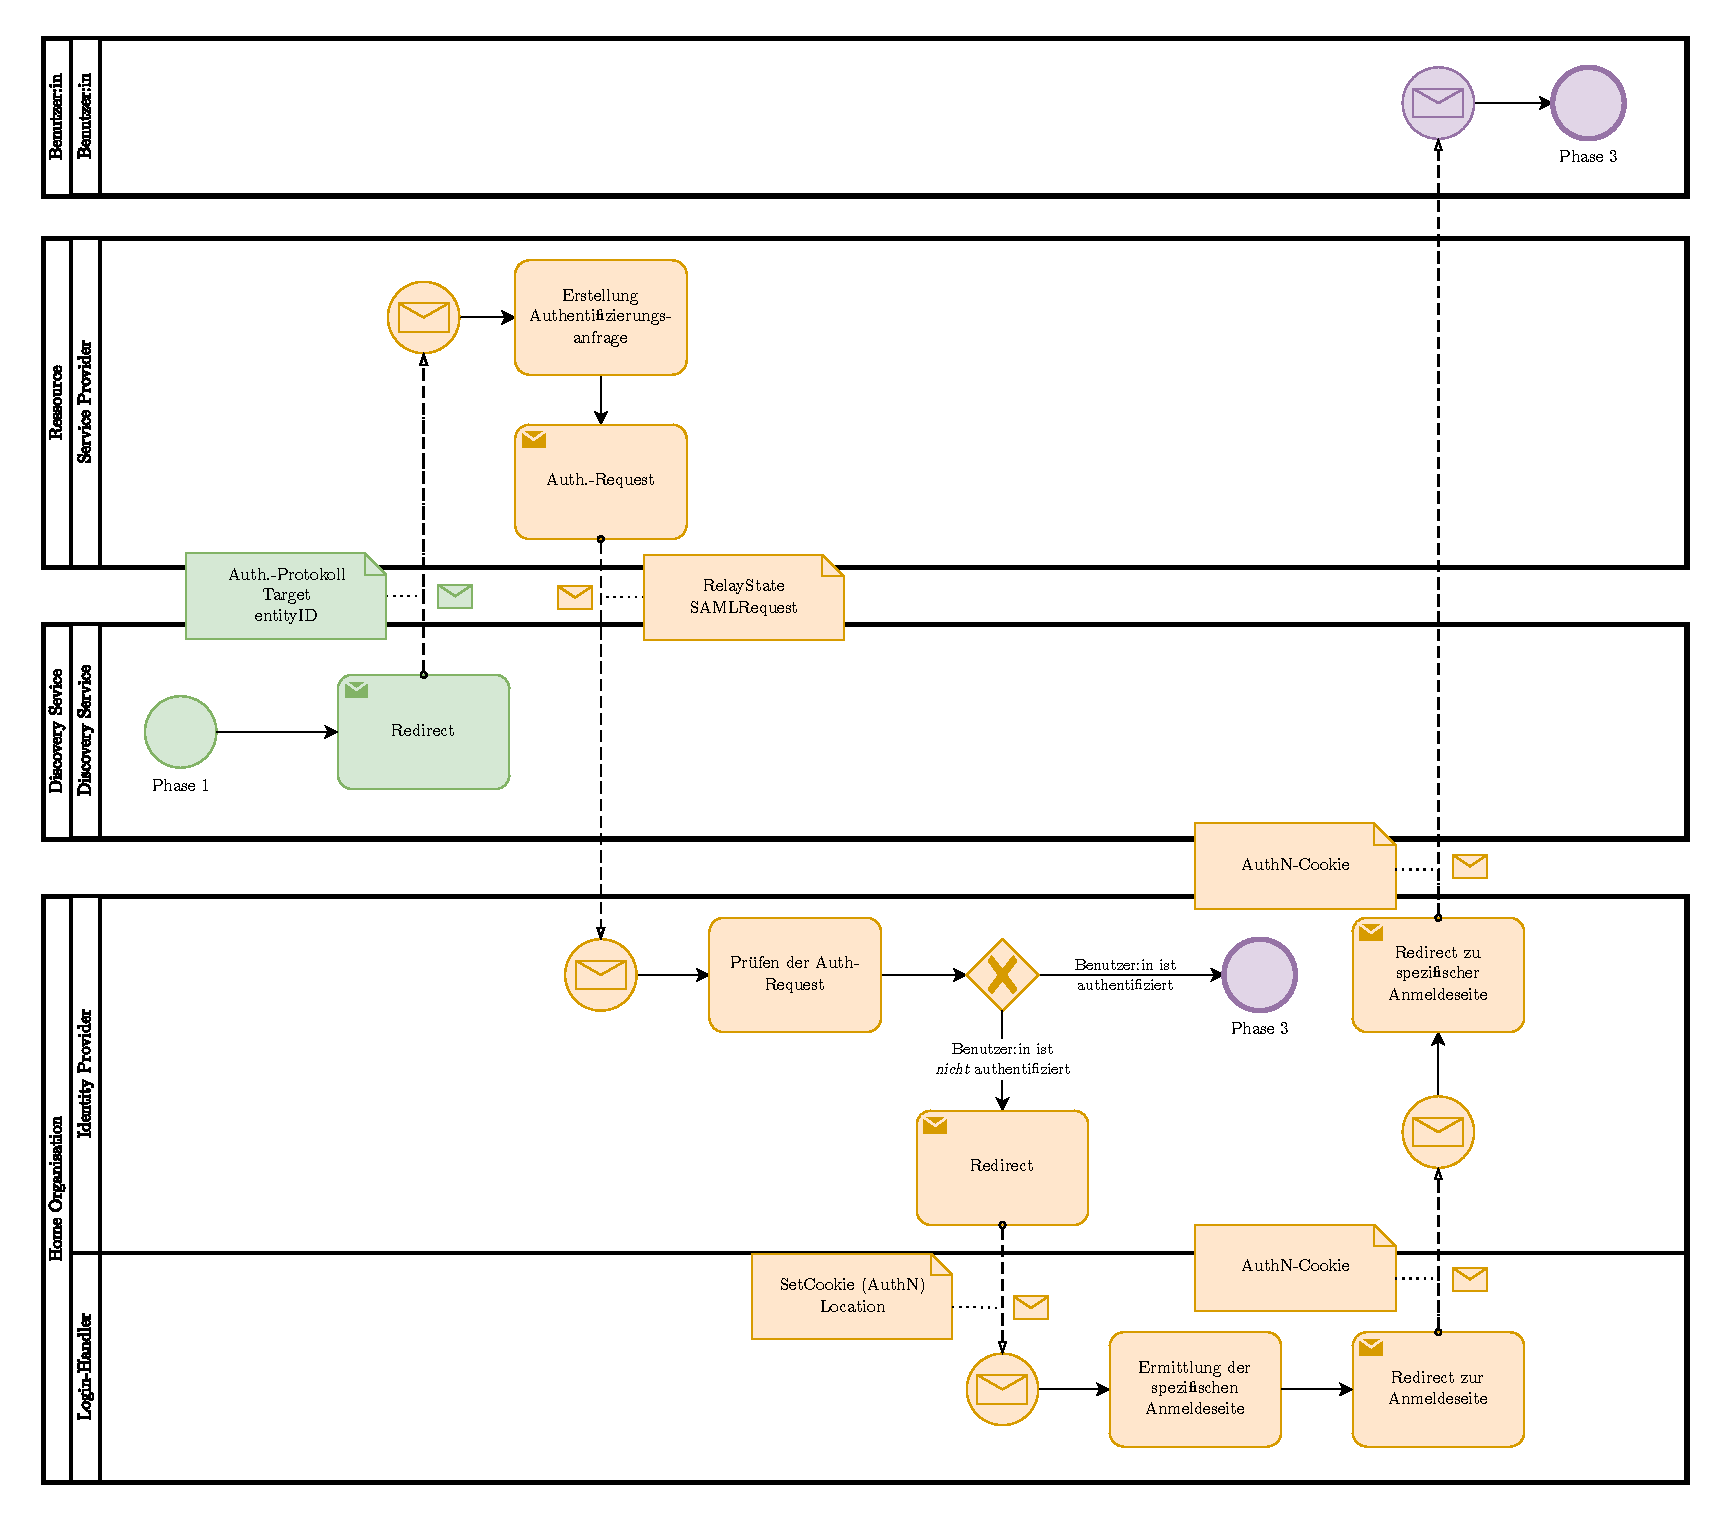
\includegraphics[height=0.7\paperheight]{../assets/bis_bpmn_phase_2.drawio.pdf}
        \caption{Phase 2 im Shibboleth-Prozess~\cite[vgl.][]{switchExpertDemoSWITCHaai2024a}}
    \end{figure}
\end{frame}


\begin{frame}{Phase 3: Authentifizierung, Autorisierung \& Ressourcenzugriff}
    \only<beamer>{
        \framezoom<1><2>[border](3.0cm,2.75cm)(3.8cm,1.3cm)
        \framezoom<1><3>[border](2.9cm,4cm)(4.9cm,3.0cm)
        \framezoom<1><4>[border](2.6cm,0.35cm)(3.7cm,1.3cm)
        \framezoom<1><5>[border](3.0cm,1.6cm)(3.8cm,1.3cm)
    }

    \begin{figure}
        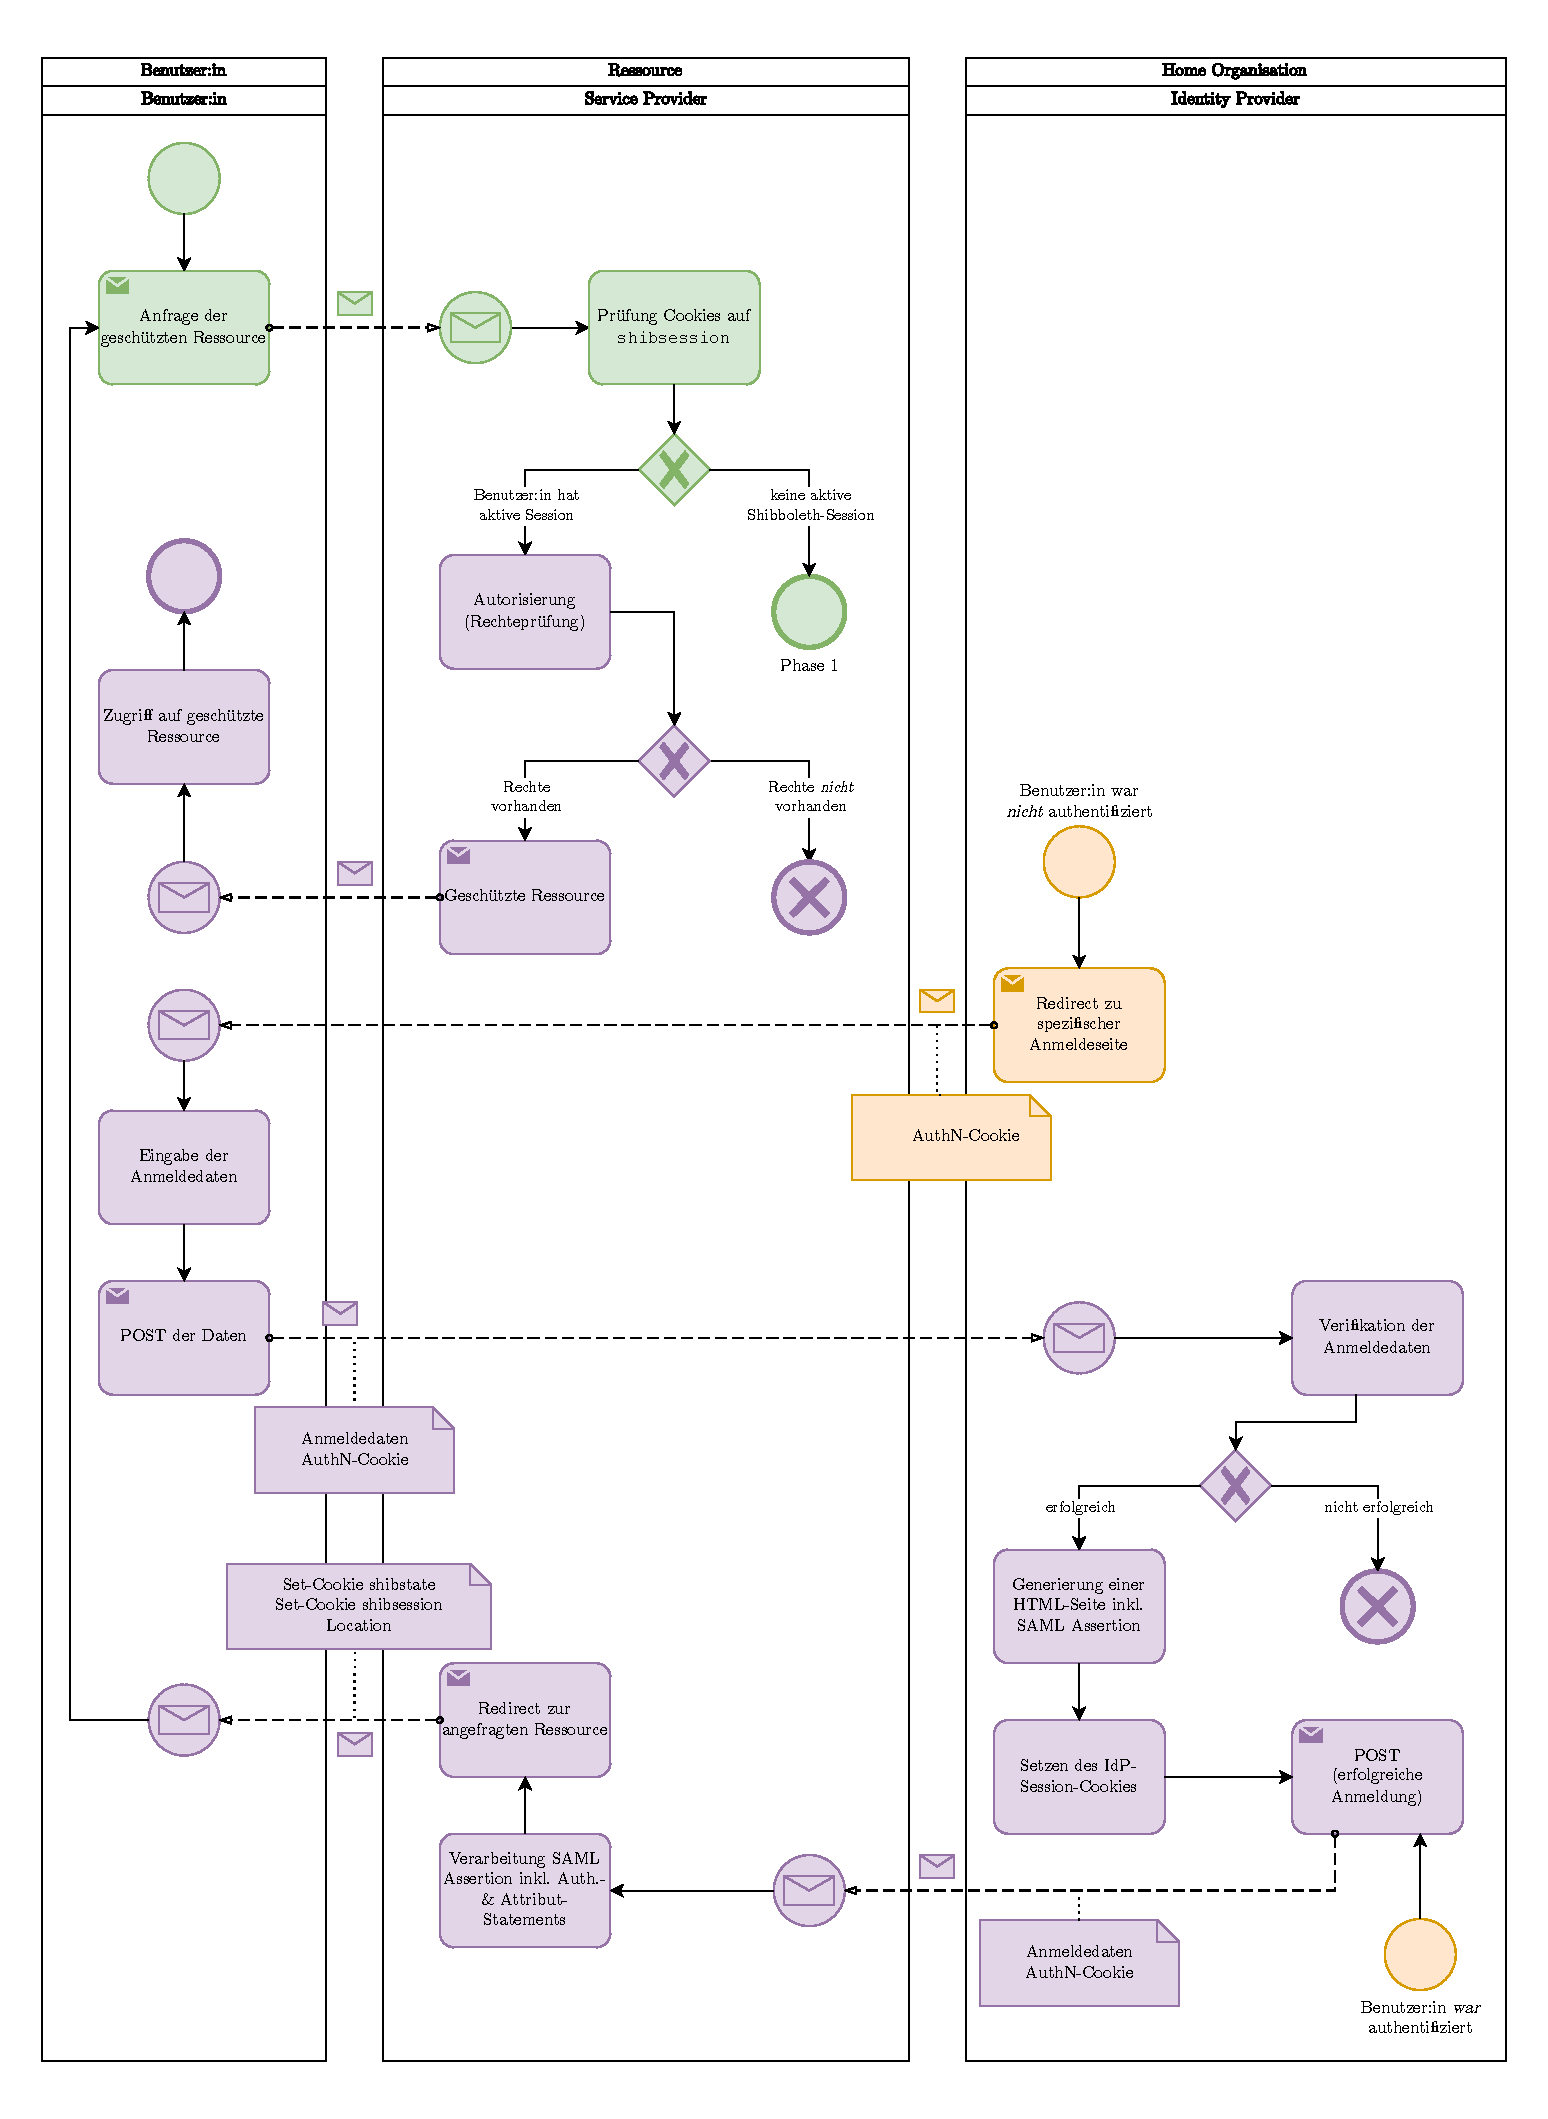
\includegraphics[height=0.7\paperheight]{../assets/bis_bpmn_phase_3.drawio.pdf}
        \caption{Phase 3 im Shibboleth-Prozess~\cite[vgl.][]{switchExpertDemoSWITCHaai2024a}}
    \end{figure}
\end{frame}
